\section{Basics of data science}
\setcounter{figure}{0}

\subsection{Data science pipeline}
First, we are going to look at how data is processed in terms of the \textbf{data science pipeline} as it can be seen in \ref{fig:1_pipeline}. 

\begin{figure}[H]
  \centering
  \begin{sidenote}{Data science pipeline}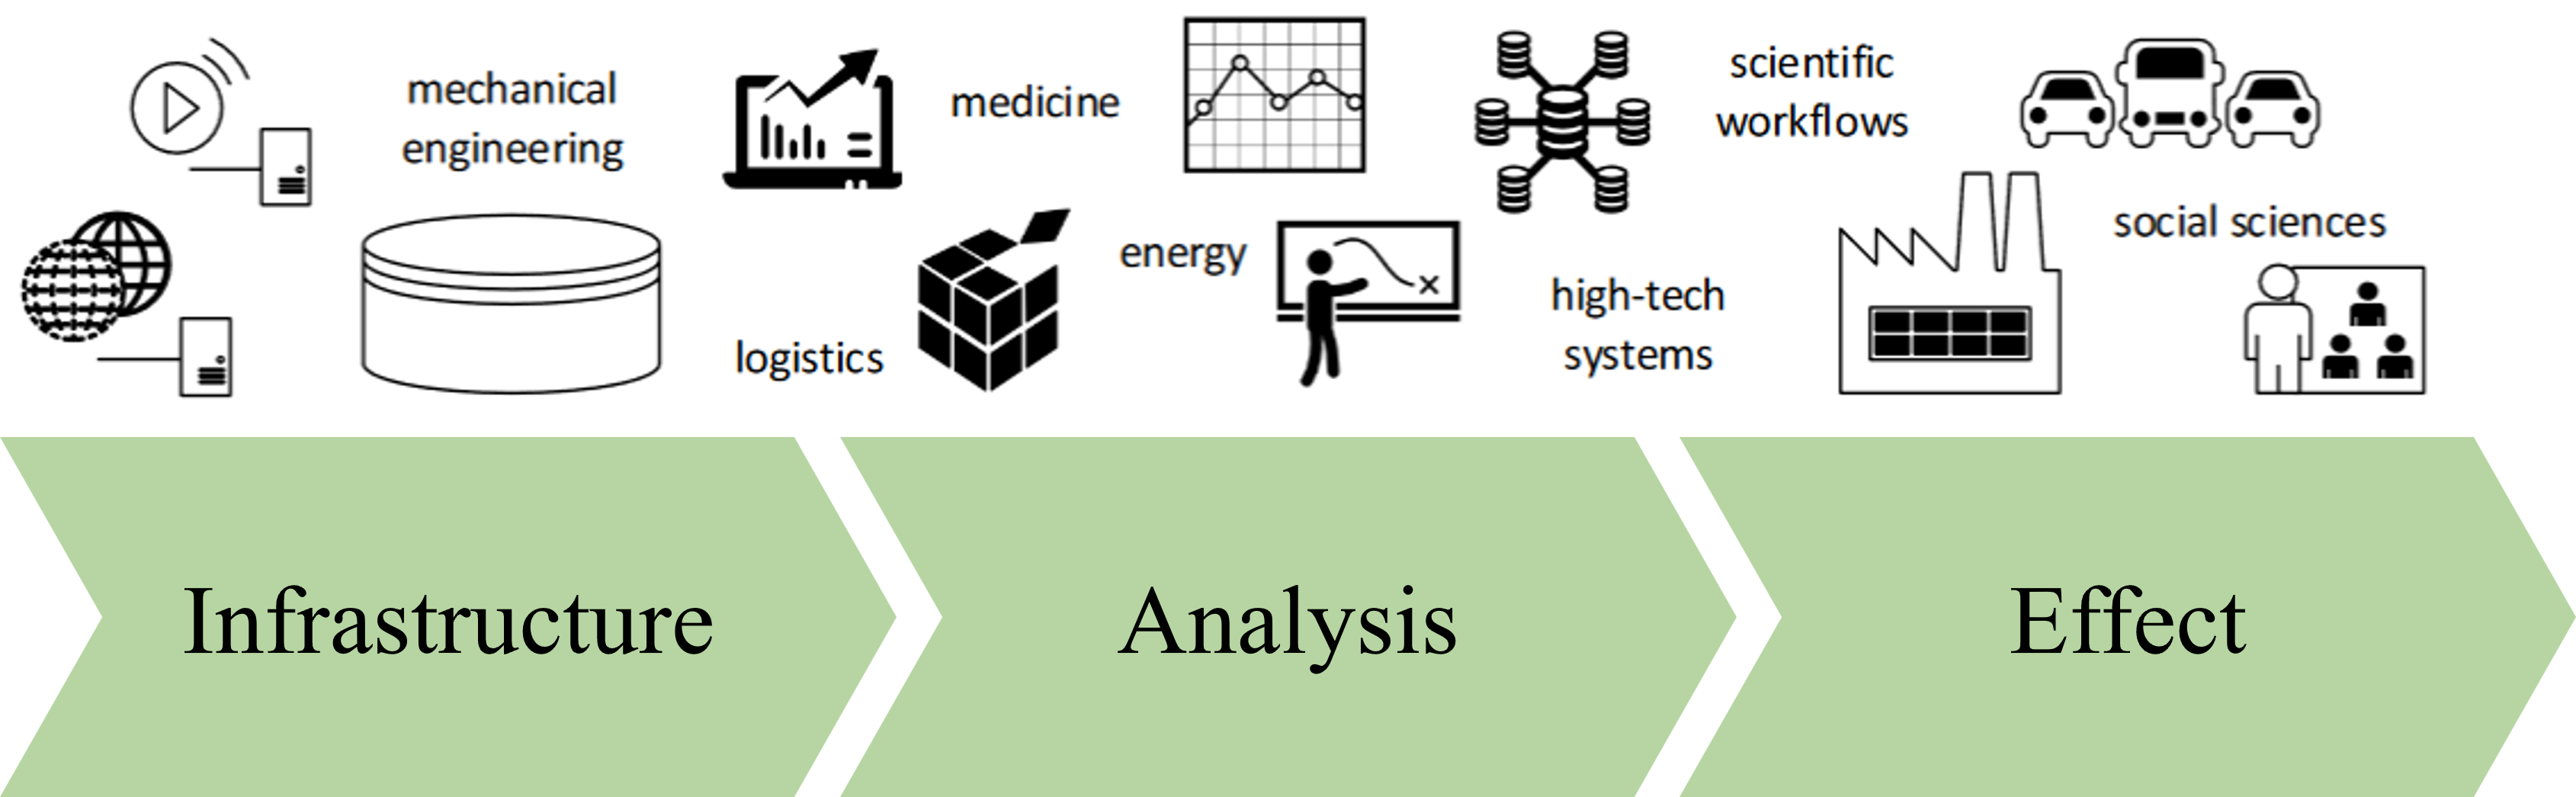
\includegraphics[width=0.9\textwidth]{assets/basics/pipeline.png}\end{sidenote}
  \caption{Pipeline of data science}
  \label{fig:1_pipeline}
\end{figure}

Let's look at the individual components. The first step to pay attention to when wanting to handle data is the \begin{sidenote}{Infrastructure}\textbf{infrastructure}\end{sidenote} with the keywords \textbf{"volume and velocity"}. The main challenge is making things scalable and instant. Important terms are for example:
\begin{itemize}
  \item Instrumentation
  \item Big data infrastructures, distributed systems
  \item Data engineering (databases and data management)
  \item Programming
  \item Security
  \item Scalability, responsiveness
\end{itemize}

Next, we have the step of the actual \begin{sidenote}{Analysis}\textbf{analysis}\end{sidenote} concerned with \textbf{extracting knowledge} from data. The core challenge can be put as providing answers to known and unknown unknowns. Important terms are for example:
\begin{itemize}
  \item Statistics
  \item Data and process mining
  \item Machine learning, artificial intelligence
  \item Operations research
  \item Algorithms
  \item Visualization
\end{itemize}

Finally, we also need to be concerned with the \begin{sidenote}{Effects}\textbf{effect}\end{sidenote} of our results on people, organizations, and society. The main challenge of this pipeline step is to do \textbf{responsibly} perform data handling. Important terms are for example:
\begin{itemize}
  \item Ethics and privacy
  \item IT law
  \item Human-technology interaction
  \item Operations management
  \item Business models
  \item Entrepreneurship
\end{itemize}

This course will look into all the steps of the pipeline, but the main focus lies on the data analysis.


\subsection{Four generic data science questions}
Important to answering all these questions is to keep attention to all three pipeline steps, so not only what analysis we need to perform to answer them, but also how we collect our input (data) and how to deal with our output (result).

Nonetheless, here are the four generic data science questions, with variety in terms of difficulty and predicting the future:
\begin{enumerate}
  \item \textbf{What} happened?
  \item \textbf{Why} did it happen?
  \item What will happen in the \textbf{future}?
  \item What is the \textbf{best} that can happen?
\end{enumerate}


\subsection{Types of data}
Now that we know that we have some kind of data as our input, we need to take a look at what this data can look like. Generally speaking, there are two types:
\begin{itemize}
  \item \begin{sidenote}{Structured data}Structured data\end{sidenote} like age, time, gender, class, etc., and
  \item \begin{sidenote}{Unstructured data}Unstructured data\end{sidenote} like text, audio, video, etc.
\end{itemize}

For \textbf{structured data} we have a further subdivision into structured data types. The data types depicted in \ref{fig:1_structured_data} will be described in detail.

\begin{figure}[H]
  \centering
  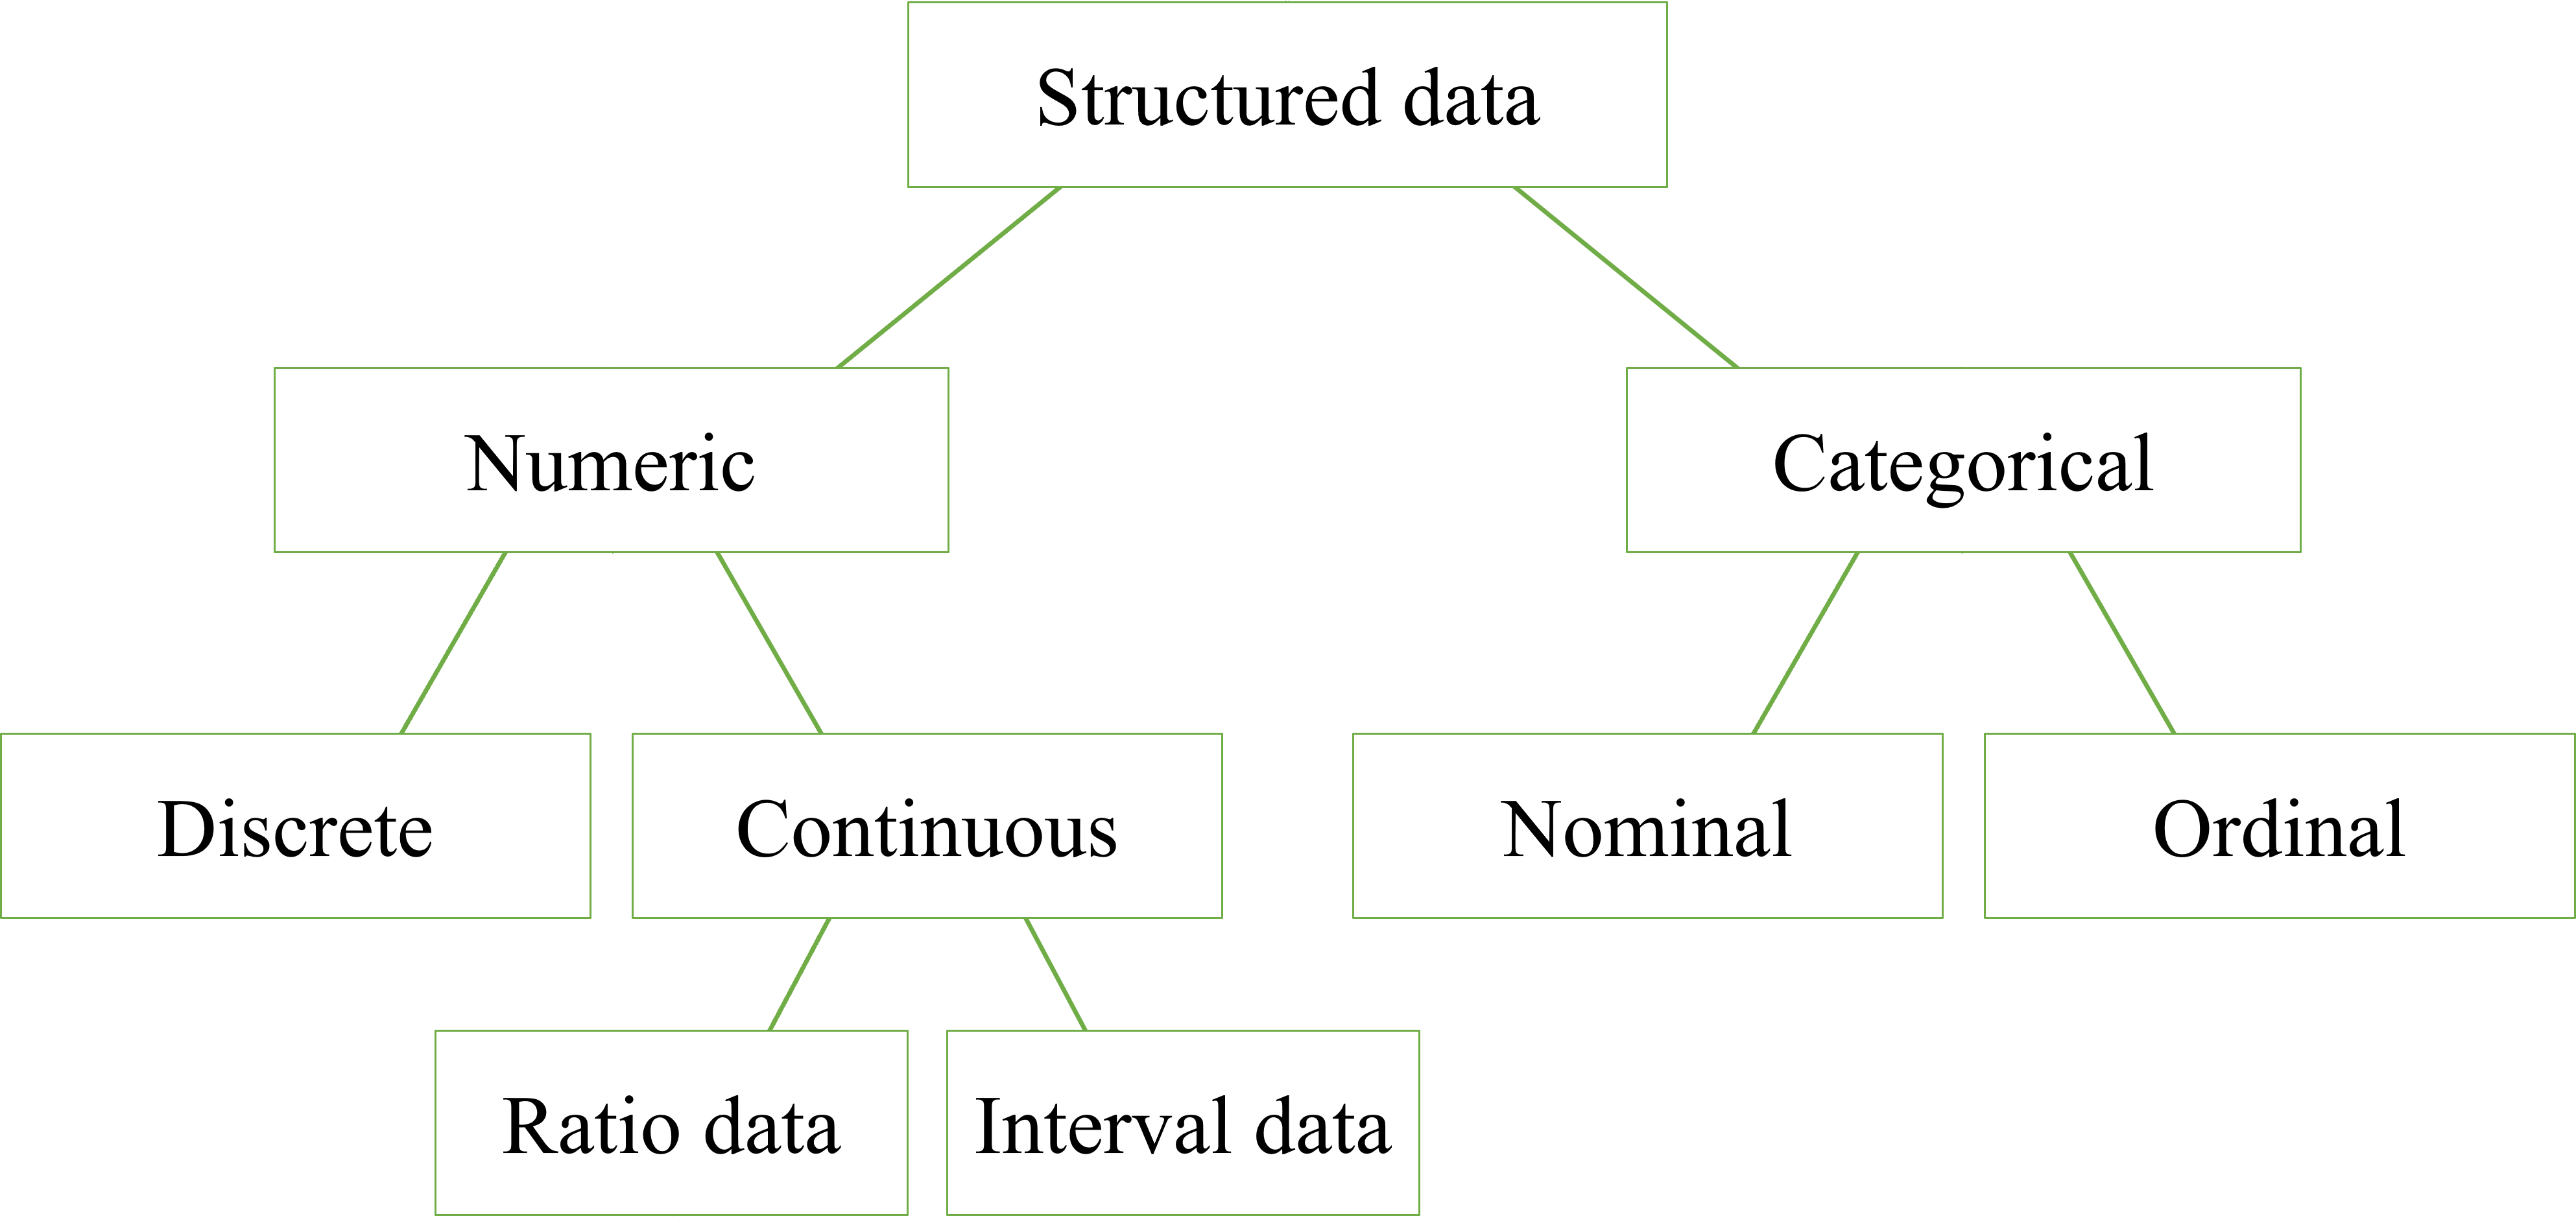
\includegraphics[width=0.6\textwidth]{assets/basics/structured_data.png}
  \caption{Overview structured data types}
  \label{fig:1_structured_data}
\end{figure}

\begin{itemize}
  \item \begin{sidenote}{Categorical data}\textbf{Categorical} data\end{sidenote} can be stored and identified based on names or labels given to them and is also known as "qualitative" data. Matching can be applied, where data is grouped based on similarities.
  
  \item Concretely, \begin{sidenote}{Nominal data}\textbf{nominal} data\end{sidenote} or naming data has a label and its characteristic similar to a noun and doesn't imply an order.
  \begin{itemize}
    \item {\footnotesize\color{ForestGreen}Example: name, color=red, country=NL}
  \end{itemize}
  
  \item \begin{sidenote}{Ordinal data}\textbf{Ordinal} data\end{sidenote} on the other hand is ranked, ordered, or used on a rating scale. This means, you can count and order ordinal data but are not able to measure it.
  \begin{itemize}
    \item {\footnotesize\color{ForestGreen}Example: risk=medium, score=good}
  \end{itemize}
  
  \item In contrast to categorical data, we also have \begin{sidenote}{Numerical data}\textbf{numerical} data\end{sidenote} referring to data in the form of numbers instead of another language or descriptive form. It is also known as "quantitative" data. Important is the ability to be statistically and arithmetically calculated (allowing for $+, -, >, =, \dots$).
  
  \item One subtype of numerical data is \begin{sidenote}{Discrete data}\textbf{discrete} data\end{sidenote} representing countable items, that are collected in a list (finite or infinite).
  \begin{itemize}
    \item {\footnotesize\color{ForestGreen}Example: number of items=5, age=18}
  \end{itemize}
  
  \item Then, there's also \begin{sidenote}{Continuous data}\textbf{continuous} data\end{sidenote} in the form of intervals or ranges. The data represents measurements with their intervals falling on a number line (so counting isn't involved).
  
  \item Continuous data can now be further distinguished. One subtype is \begin{sidenote}{Interval data}\textbf{interval}\end{sidenote} data where the data can be measured only along a scale at equal distances from each other, so only addition and subtraction operations are allowed. There is no true zero (and hence no $\cdot, /$).
  \begin{itemize}
    \item {\footnotesize\color{ForestGreen}Example: data=11-11-2018, temp=18.5°C}
  \end{itemize}
  
  \item And finally, we have \begin{sidenote}{Ratio data}\textbf{ratio} data\end{sidenote} describing measurement with a defined (true) zero point.
  \begin{itemize}
    \item {\footnotesize\color{ForestGreen}Example: dropout=33\%, speed=128.34km/h}
  \end{itemize}
\end{itemize}

For \textbf{unstructured data}, we just take the raw data and interpret it as a stream of bits. This goes for text, audio, images, signals, and videos exactly the same. Examples can be seen in \ref{fig:1_unstructured_data}.

\begin{figure}[H]
  \centering
  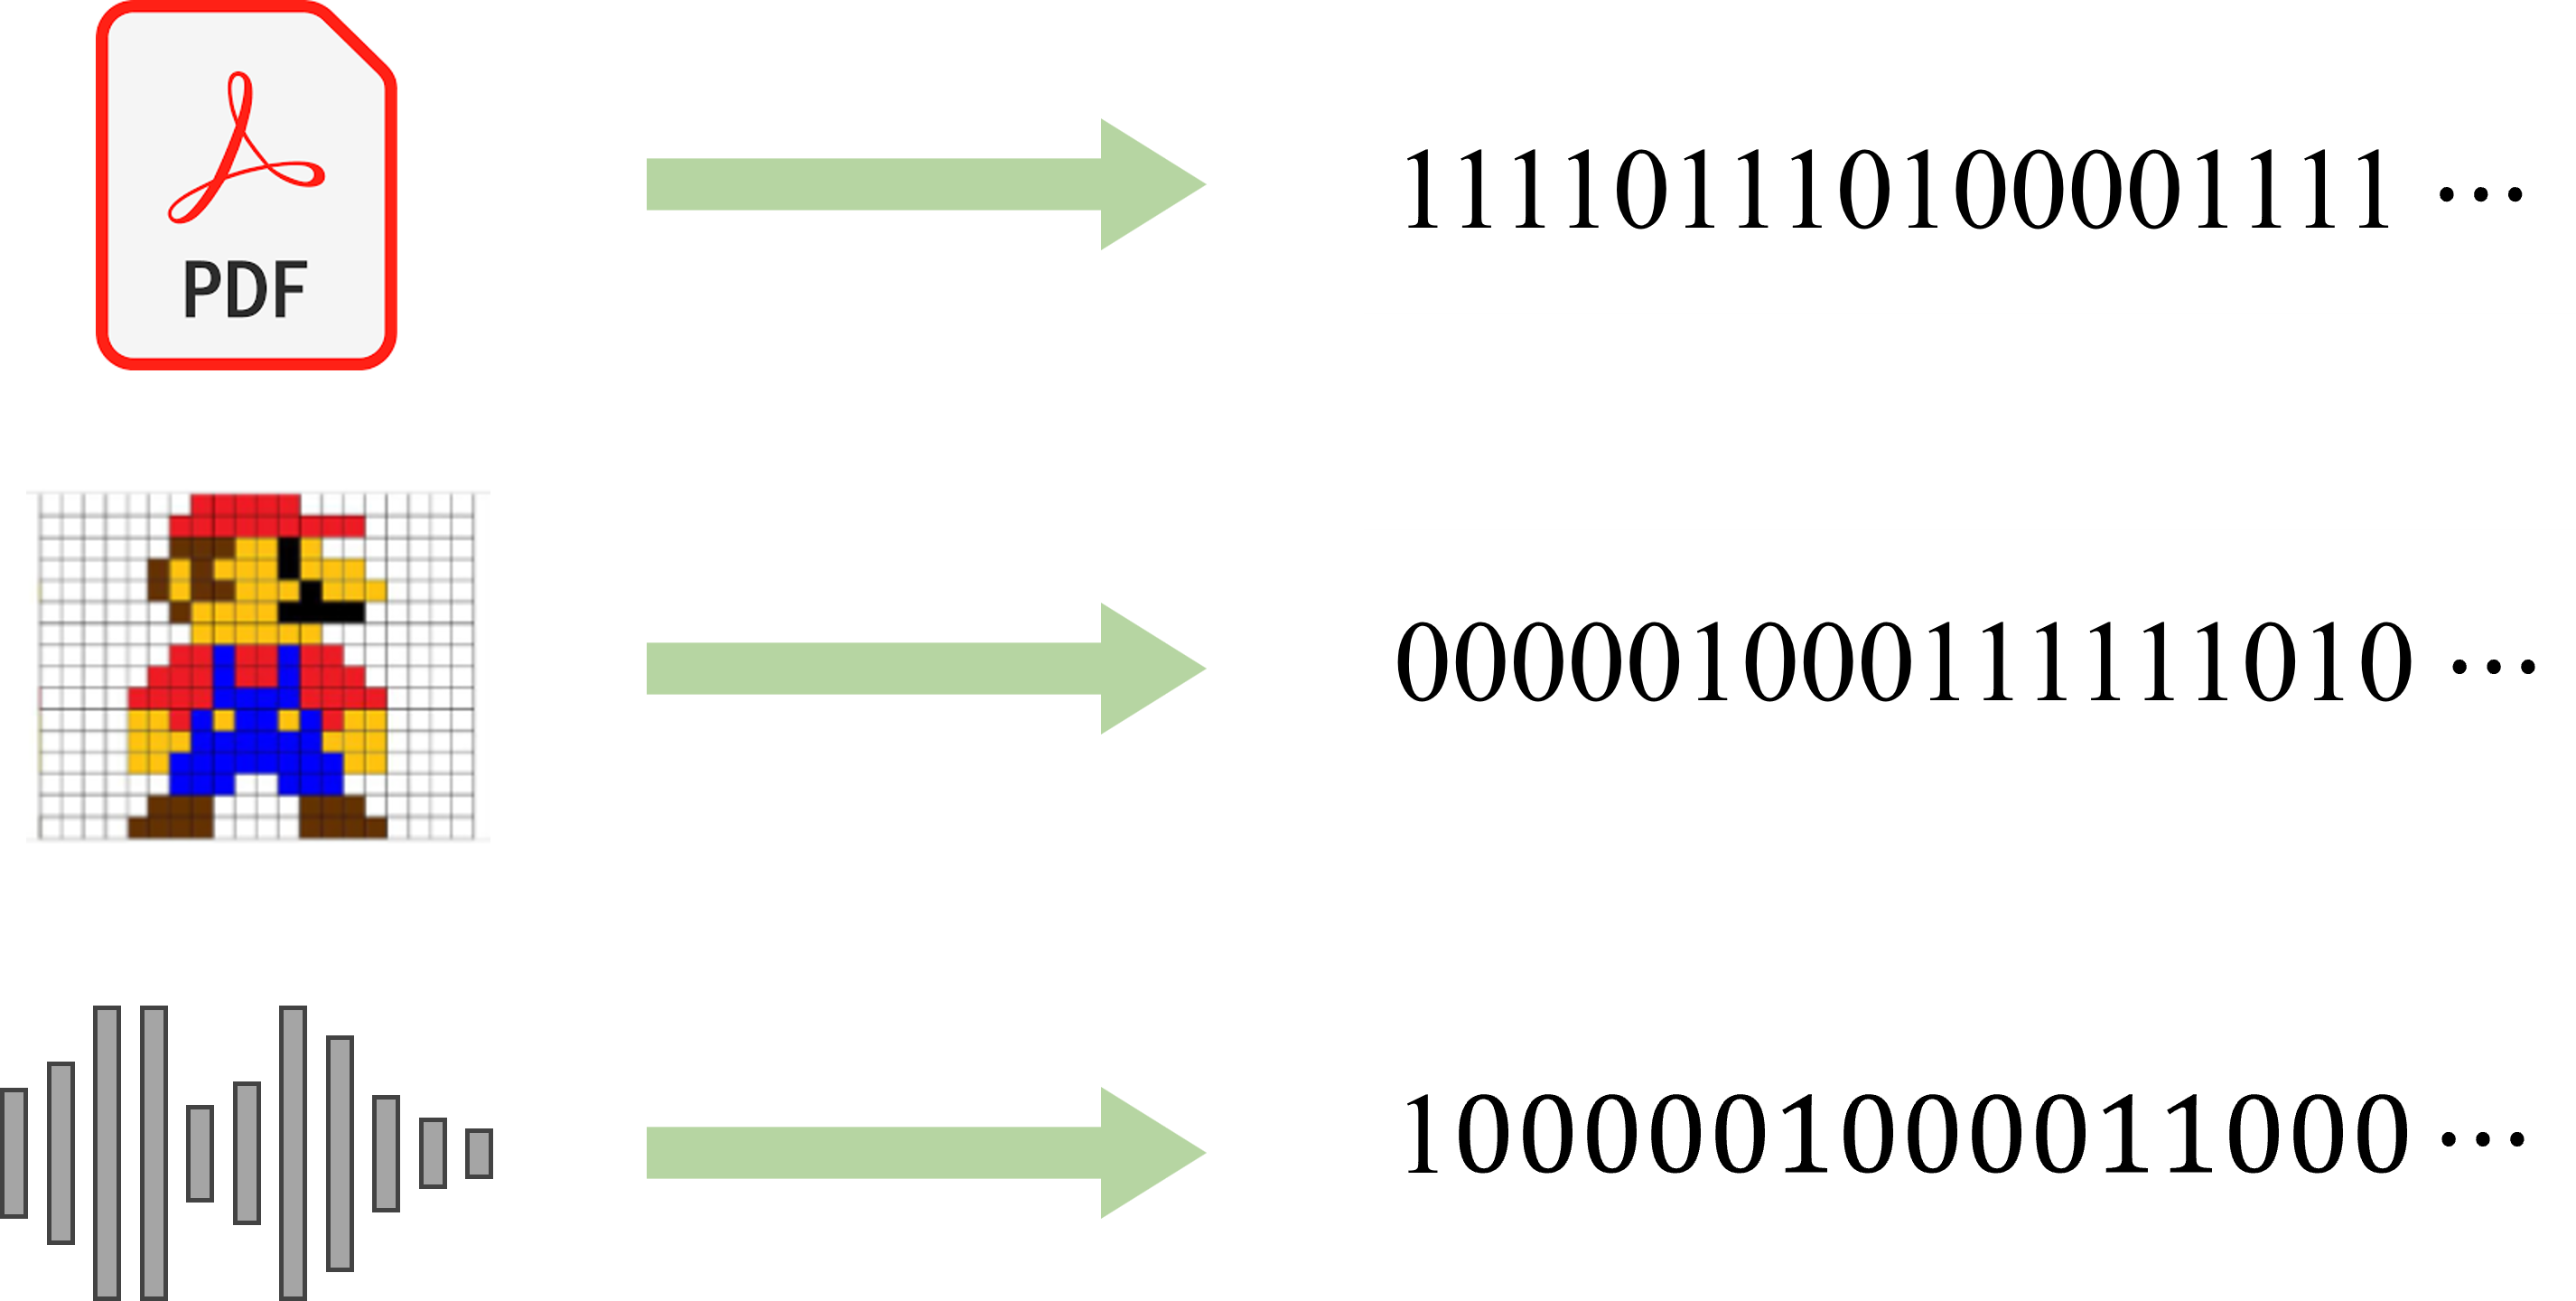
\includegraphics[width=0.6\textwidth]{assets/basics/unstructured_data.png}
  \caption{Input for unstructured data}
  \label{fig:1_unstructured_data}
\end{figure}

Data can now be stored and ordered together by putting it into \begin{sidenote}{Tabular data}\textbf{tables}\end{sidenote}. Concretely, columns represent different features (can be different kinds of data types) whereas rows describe data instances. Examples can be seen in \ref{fig:1_table_data}.

\begin{figure}[H]
  \centering
  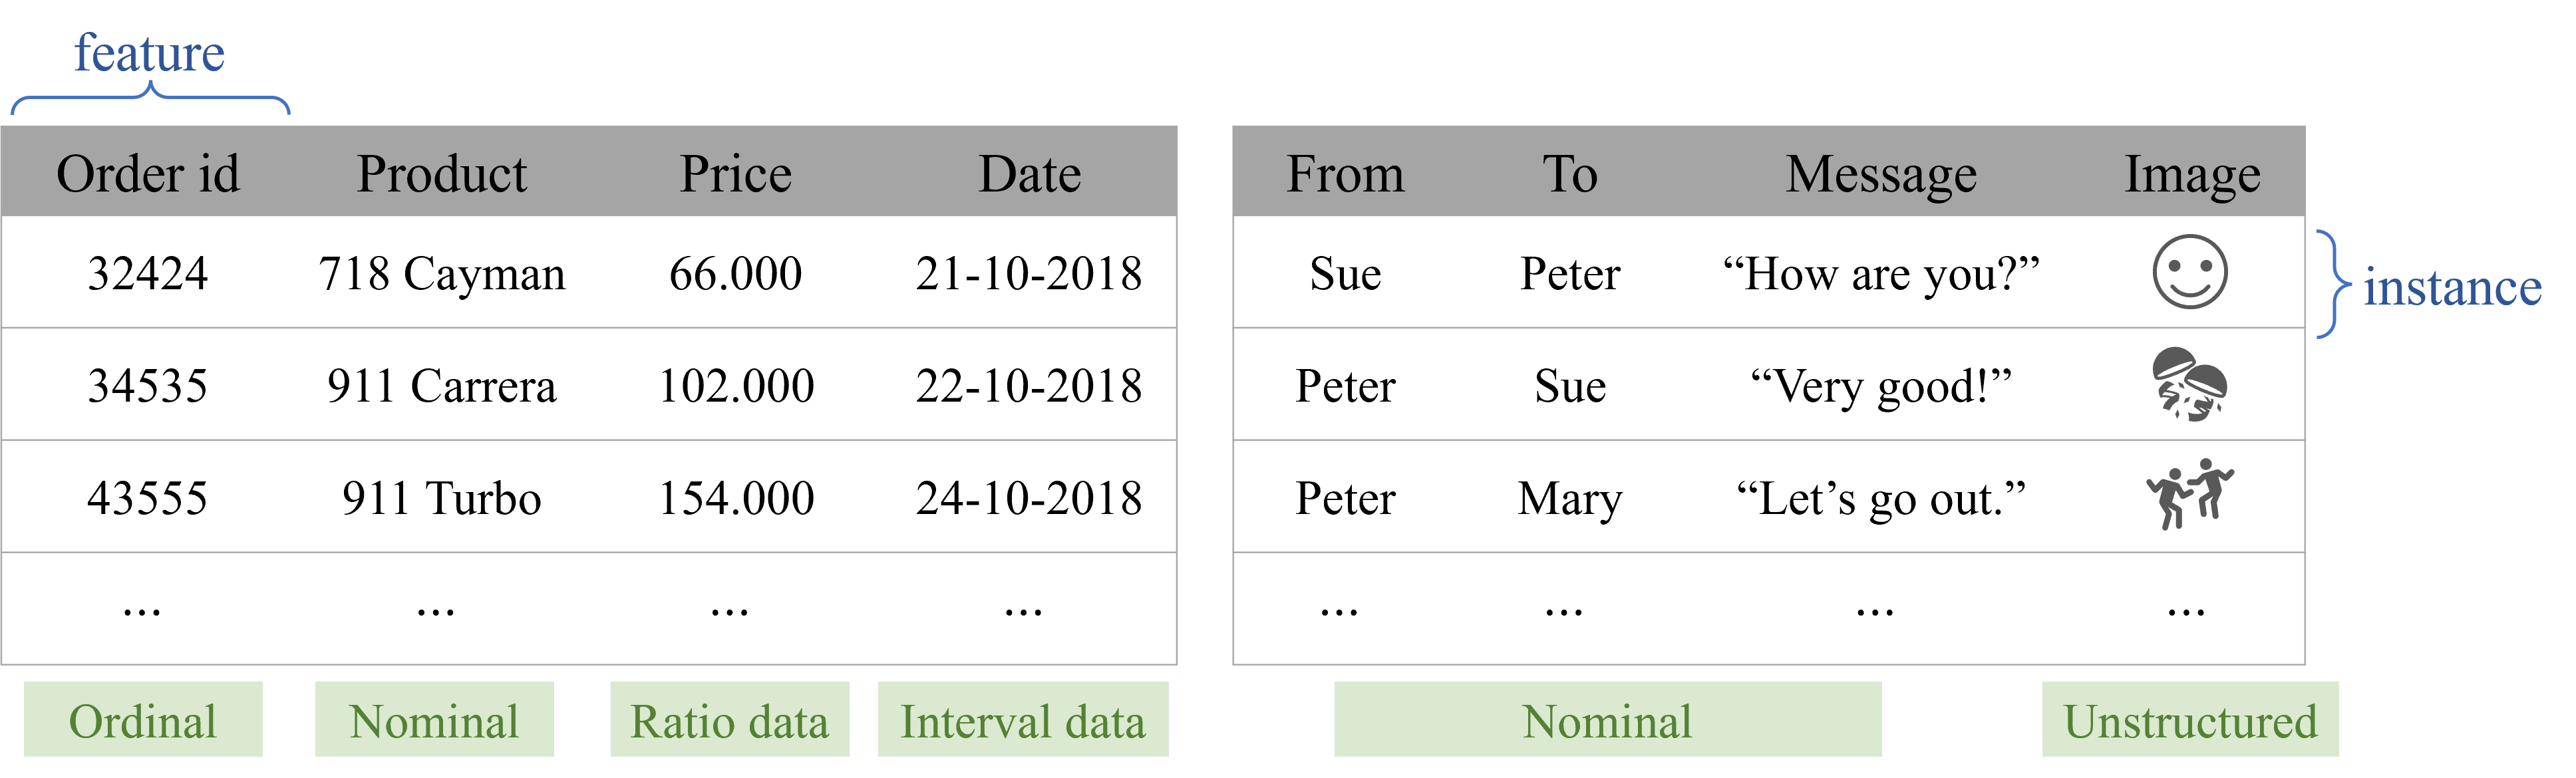
\includegraphics[width=0.9\textwidth]{assets/basics/table_data.png}
  \caption{Table data with data types}
  \label{fig:1_table_data}
\end{figure}

